\problemname{Mötesplats}
$N$ stycken vänner bor på var sin nod i ett träd med $N$ noder, där $N$ är \textbf{udda}.
Ett \emph{träd} är en sammanhängande graf med exakt $N-1$ kanter.

Vännerna vill nu alla träffas på en nod i trädet.
De har kommit fram till att de vill mötas på den noden som minimerar
summan av distanserna till vännerna, och har frågat dig om du kan hjälpa dem att
hitta denna optimala mötesplats.
\emph{Distansen} $\text{dist}(a,b)$ mellan två noder $a$ och $b$ i trädet är antalet
kanter på vägen mellan $a$ och $b$.
Så formellt sett vill du hitta noden $x$ som minimerar
$\sum_{i=1}^{n} \text{dist}(x,i)$.

Detta tänker du är ett lätt problem, och börjar genast koda en lösning.
Men det finns en twist!
Vännerna har dåligt minne och kommer inte ihåg hur trädet ser ut.
Dock kommer de ihåg följande: givet tre \textbf{olika} vänner
$a,b,c$ kan de med säkerhet säga att de brukar mötas (när det bara är dem tre) på plats
$x$, där $x$ är noden som minimerar
$\text{dist}(x,a) +\text{dist}(x,b) +\text{dist}(x,c)$.
Notera att $x$ inte nödvändigtvis är en av noderna $a,b$ eller $c$.

I detta problem läser du alltså inte in grafen direkt i indatan,
utan får istället fråga upp till $Q-1$ frågor på formen:
\emph{Var brukar vännerna $a,b,c$ mötas?}
Med hjälp av dessa frågor vill du hitta
den optimala mötesplatsen.

\begin{figure}[!h]
\begin{center}
  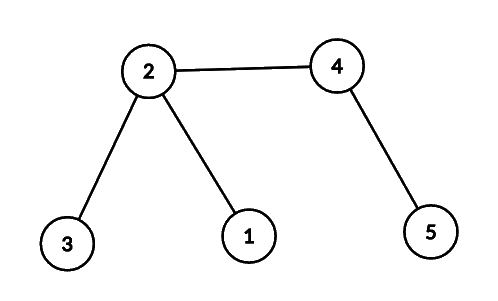
\includegraphics[width=7cm]{sample.png}
\end{center}
  \caption{Illustration av trädet i exempelfallet. Nod 2 är den optimala mötesplatsen.}
\end{figure}

\section*{Interaktion}

I första raden av indatan finns två heltal $N$ och $Q$,
antalet noder i trädet och antalet queries du får göra.
Det är garanterat att $N$ är udda och att $Q = 500\,000$ i alla testfall.

Sedan får du göra följande typer av queries:
\begin{itemize}
    \item Skriv ut en rad med ``\verb|? a b c|'' där $1\le a,b,c\le N$ är $3$ \textbf{olika} vänner.
    Därefter kommer domarprogrammet svara med en rad med ett heltal $x$ som du ska läsa in
    ($1\le x\le N$), noden som minimerar $\text{dist}(x,a) +\text{dist}(x,b) +\text{dist}(x,c)$.
  \item Skriv ut en rad med ``\verb|! x|'' där $1\le x\le N$ är den optimala mötesplatsen.
    Efter att du skrivit ut detta ska ditt program avsluta utan att skriva ut något mer. 
    Om $x$ är noden som minimerar $\sum_{i=1}^{n} \text{dist}(x,i)$ får du \textit{Accepted} på testfallet, annars \textit{Wrong Answer}.
\end{itemize}
Om du gör fler än $Q$ queries (inklusive den sista på formen ``\verb|! x|'')
kommer ditt program avslutas och du får \textit{Wrong Answer} på testfallet.

\textbf{Se till att flusha outputen efter varje query}, annars kan du få \textit{Time Limit Exceeded}.
I C++ kan detta göras med exempelvis \texttt{cout << flush}
eller \texttt{fflush(stdout)};
i Python med \texttt{stdout.flush()};
och i Java med \texttt{System.out.flush()}.

\section*{Poängsättning}
Din lösning kommer att testas på en mängd testfallsgrupper.
För att få poäng för en grupp så måste du klara alla testfall i gruppen.


\noindent
\begin{tabular}{| l | l | l |}
  \hline
  Grupp & Poängvärde & Gränser \\ \hline \hline
  $1$   & $10$        & $3 \le N\le 99$ och alla noder har grad högst 2, dvs trädet är en linje \\ \hline
  $2$   & $12$        & $3 \le N\le 999$ och alla noder har grad högst 2, dvs trädet är en linje \\ \hline
  $3$   & $21$        & $3 \le N\le 24\,999$ och alla noder har grad högst 2, dvs trädet är en linje \\ \hline \hline
  $4$   & $14$        & $3 \le N\le 99$ \\ \hline
  $5$   & $15$        & $3 \le N\le 999$ \\ \hline
  $6$   & $28$        & $3 \le N\le 24\,999$ \\ \hline
\end{tabular}
